% Editable native annotations around unchanged verified IDE photographs.
\par
\begin{figure}[htbp]
  \centering
  \newsavebox{\MARSmatmulcomparisonscalarcacheBox}
  \sbox{\MARSmatmulcomparisonscalarcacheBox}{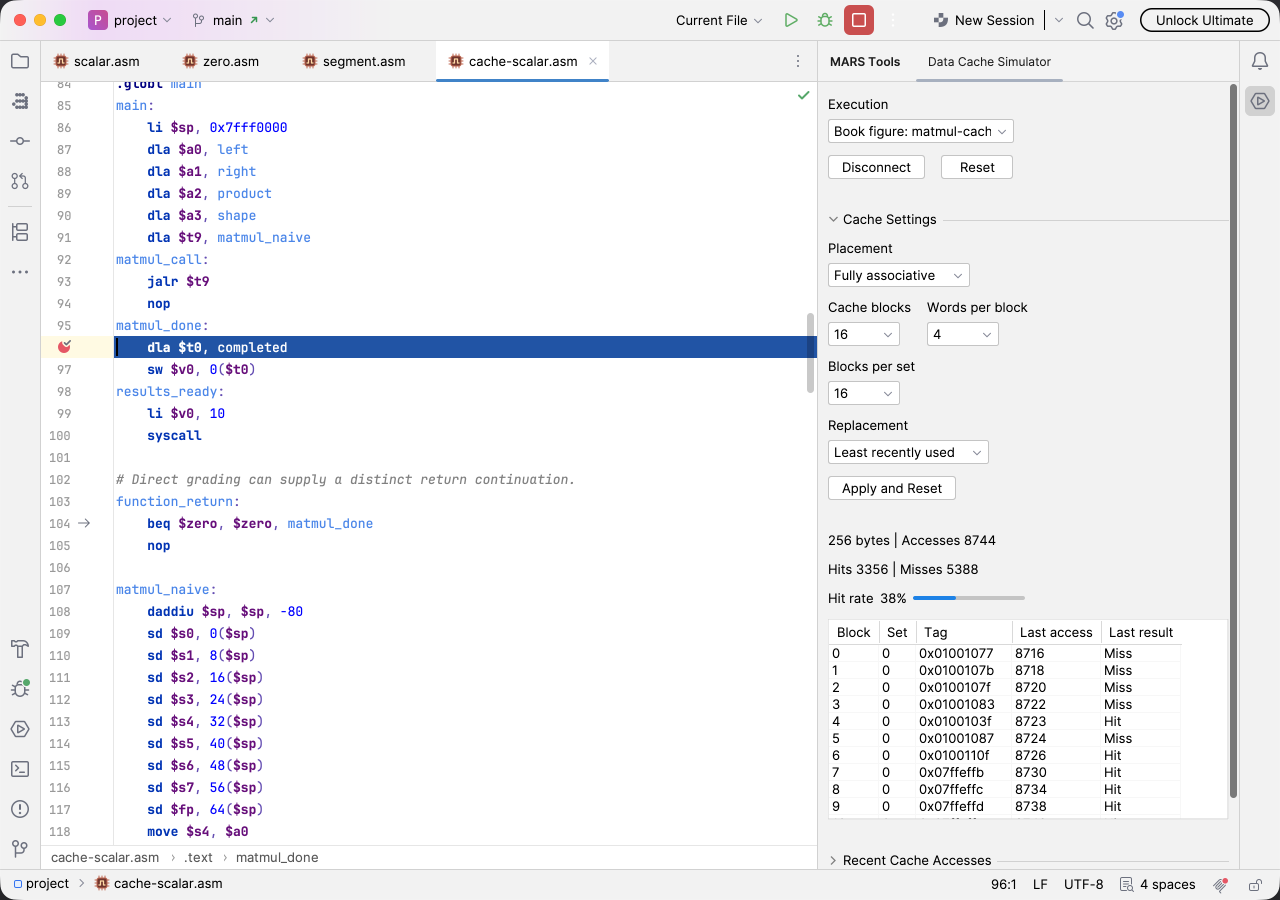
\includegraphics[artifact]{book/captures/022-blocked-matmul/f04/scalar-cache.png}}
  \newsavebox{\MARSmatmulcomparisontiledcacheBox}
  \sbox{\MARSmatmulcomparisontiledcacheBox}{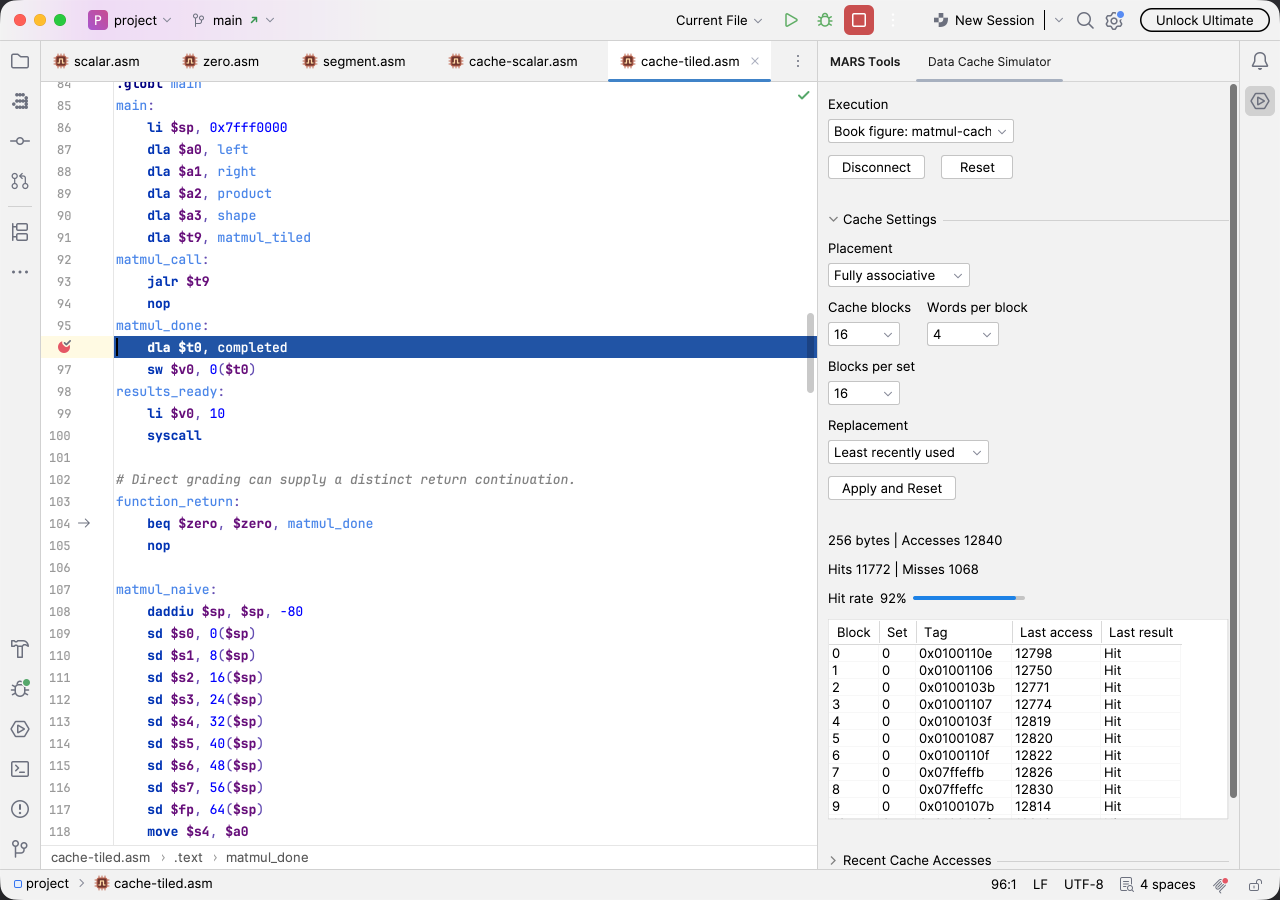
\includegraphics[artifact]{book/captures/022-blocked-matmul/f04/tiled-cache.png}}
  \newsavebox{\MARSmatmulcomparisonscalarproductBox}
  \sbox{\MARSmatmulcomparisonscalarproductBox}{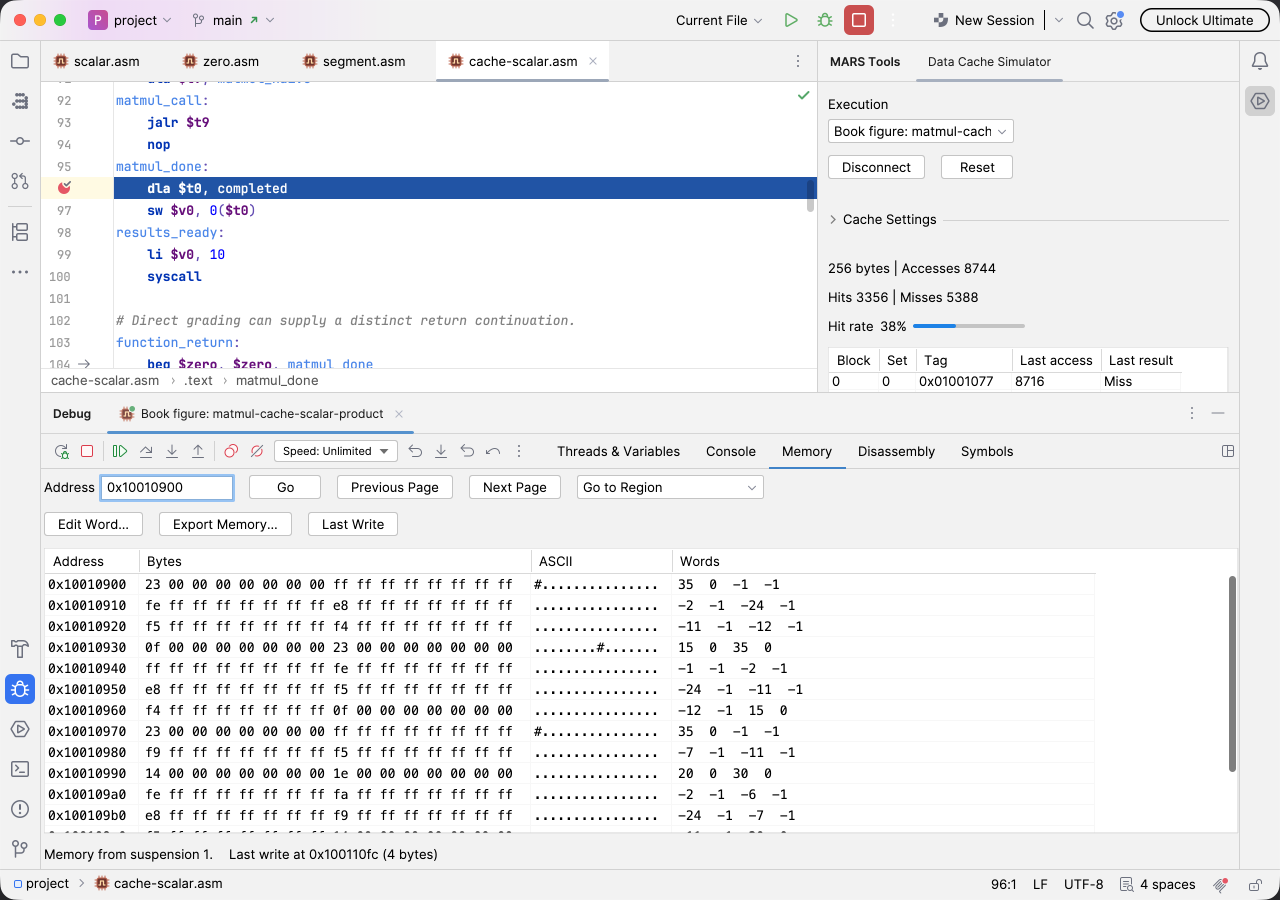
\includegraphics[artifact]{book/captures/022-blocked-matmul/f04/scalar-product.png}}
  \newsavebox{\MARSmatmulcomparisontiledproductBox}
  \sbox{\MARSmatmulcomparisontiledproductBox}{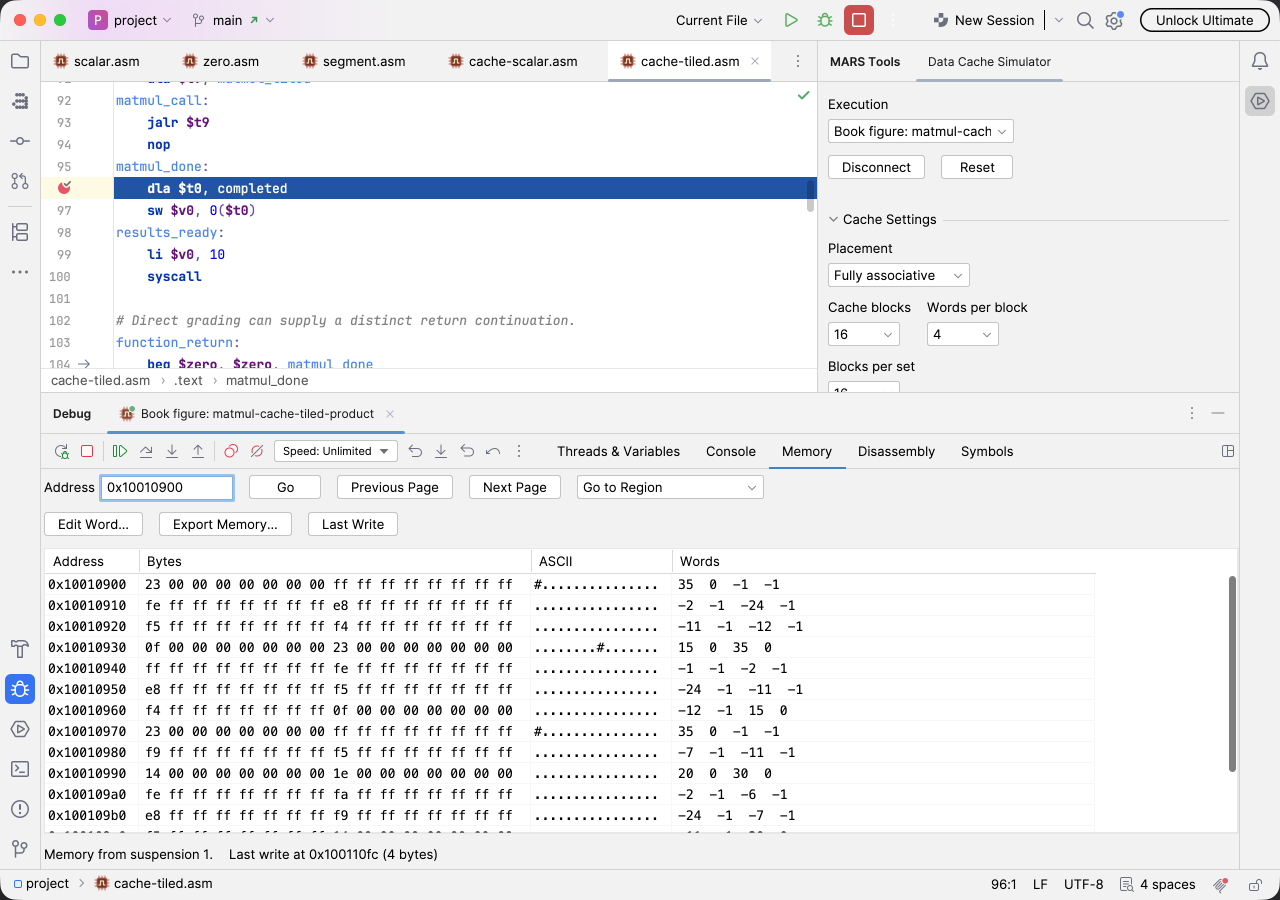
\includegraphics[artifact]{book/captures/022-blocked-matmul/f04/tiled-product.png}}
  \edef\MARSmatmulcomparisonscalarstatsLeft{\the\dimexpr0.644531250\wd\MARSmatmulcomparisonscalarcacheBox\relax}
  \edef\MARSmatmulcomparisonscalarstatsBottom{\the\dimexpr0.323333333\ht\MARSmatmulcomparisonscalarcacheBox\relax}
  \edef\MARSmatmulcomparisonscalarstatsRight{\the\dimexpr0.037500000\wd\MARSmatmulcomparisonscalarcacheBox\relax}
  \edef\MARSmatmulcomparisonscalarstatsTop{\the\dimexpr0.588888889\ht\MARSmatmulcomparisonscalarcacheBox\relax}
  \edef\MARSmatmulcomparisontiledstatsLeft{\the\dimexpr0.644531250\wd\MARSmatmulcomparisontiledcacheBox\relax}
  \edef\MARSmatmulcomparisontiledstatsBottom{\the\dimexpr0.323333333\ht\MARSmatmulcomparisontiledcacheBox\relax}
  \edef\MARSmatmulcomparisontiledstatsRight{\the\dimexpr0.037500000\wd\MARSmatmulcomparisontiledcacheBox\relax}
  \edef\MARSmatmulcomparisontiledstatsTop{\the\dimexpr0.588888889\ht\MARSmatmulcomparisontiledcacheBox\relax}
  \edef\MARSmatmulcomparisonscalarproductLeft{\the\dimexpr0.034375000\wd\MARSmatmulcomparisonscalarproductBox\relax}
  \edef\MARSmatmulcomparisonscalarproductBottom{\the\dimexpr0.311111111\ht\MARSmatmulcomparisonscalarproductBox\relax}
  \edef\MARSmatmulcomparisonscalarproductRight{\the\dimexpr0.584375000\wd\MARSmatmulcomparisonscalarproductBox\relax}
  \edef\MARSmatmulcomparisonscalarproductTop{\the\dimexpr0.608888889\ht\MARSmatmulcomparisonscalarproductBox\relax}
  \edef\MARSmatmulcomparisontiledproductLeft{\the\dimexpr0.034375000\wd\MARSmatmulcomparisontiledproductBox\relax}
  \edef\MARSmatmulcomparisontiledproductBottom{\the\dimexpr0.311111111\ht\MARSmatmulcomparisontiledproductBox\relax}
  \edef\MARSmatmulcomparisontiledproductRight{\the\dimexpr0.584375000\wd\MARSmatmulcomparisontiledproductBox\relax}
  \edef\MARSmatmulcomparisontiledproductTop{\the\dimexpr0.608888889\ht\MARSmatmulcomparisontiledproductBox\relax}
  \begin{tikzpicture}[alt={Four annotated details compare scalar and tiled sixteen-by-sixteen calls at matmul_done. Both caches have capacity 256 bytes. Scalar has 8744 accesses and 5388 misses; tile four has 12840 accesses and 1068 misses. Both output details show exact doublewords 35 minus one minus two minus 24.}]
    \node[anchor=north west,inner sep=0,font=\small\bfseries] (scalarstats-title) at (6mm,0) {Scalar cache counters};
    \node[anchor=north west,inner sep=0] (scalarstats) at ([yshift=-1mm]scalarstats-title.south west) {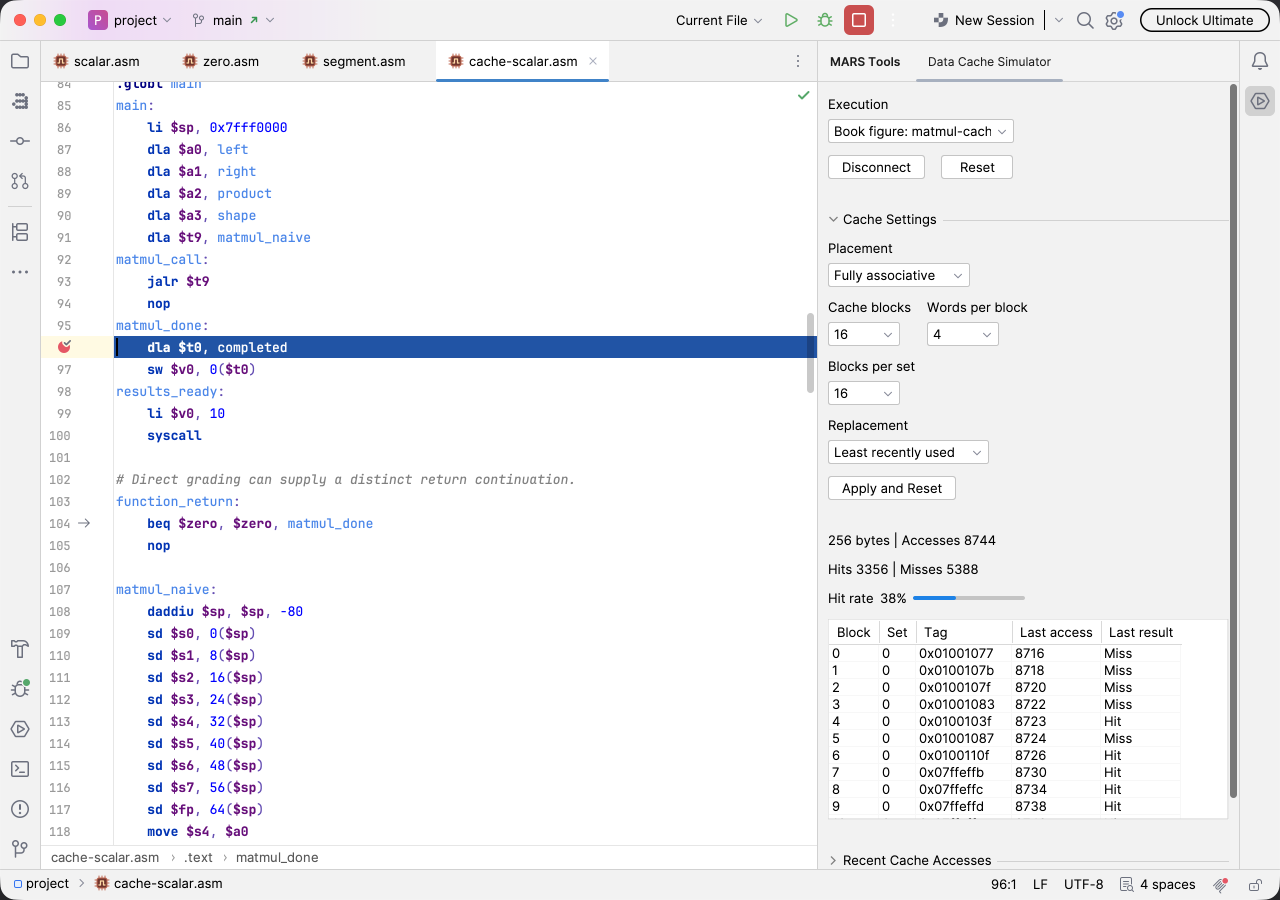
\includegraphics[width=0.84\linewidth,artifact,trim={\MARSmatmulcomparisonscalarstatsLeft{} \MARSmatmulcomparisonscalarstatsBottom{} \MARSmatmulcomparisonscalarstatsRight{} \MARSmatmulcomparisonscalarstatsTop{}},clip]{book/captures/022-blocked-matmul/f04/scalar-cache.png}};
    \begin{scope}[shift={(scalarstats.south west)},x={($(scalarstats.south east)-(scalarstats.south west)$)},y={($(scalarstats.north west)-(scalarstats.south west)$)}]
      \draw[black,line width=0.7pt] (0.007371007,0.025316456) rectangle (0.992628993,0.974683544);
      \node[draw=black,fill=white,circle,inner sep=1.5pt,font=\footnotesize] at ($(0,0.974683544)+(-3mm,0)$) {1};
    \end{scope}
    \node[anchor=north west,inner sep=0,font=\small\bfseries] (tiledstats-title) at ([yshift=-1mm]scalarstats.south west) {Tile-four cache counters};
    \node[anchor=north west,inner sep=0] (tiledstats) at ([yshift=-1mm]tiledstats-title.south west) {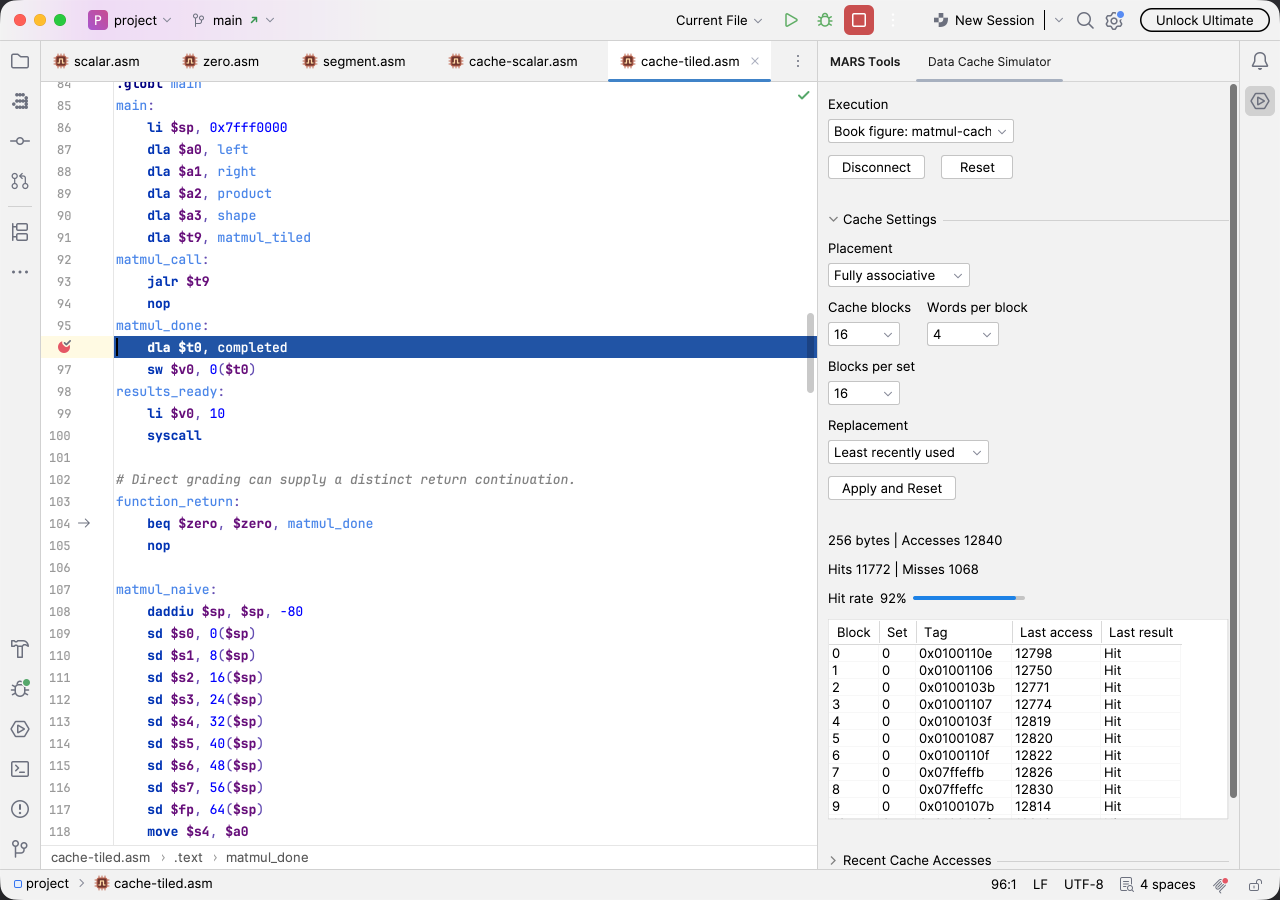
\includegraphics[width=0.84\linewidth,artifact,trim={\MARSmatmulcomparisontiledstatsLeft{} \MARSmatmulcomparisontiledstatsBottom{} \MARSmatmulcomparisontiledstatsRight{} \MARSmatmulcomparisontiledstatsTop{}},clip]{book/captures/022-blocked-matmul/f04/tiled-cache.png}};
    \begin{scope}[shift={(tiledstats.south west)},x={($(tiledstats.south east)-(tiledstats.south west)$)},y={($(tiledstats.north west)-(tiledstats.south west)$)}]
      \draw[black,line width=0.7pt] (0.007371007,0.025316456) rectangle (0.992628993,0.974683544);
      \node[draw=black,fill=white,circle,inner sep=1.5pt,font=\footnotesize] at ($(0,0.974683544)+(-3mm,0)$) {2};
    \end{scope}
    \node[anchor=north west,inner sep=0,font=\small\bfseries] (scalarproduct-title) at ([yshift=-1mm]tiledstats.south west) {Scalar output detail};
    \node[anchor=north west,inner sep=0] (scalarproduct) at ([yshift=-1mm]scalarproduct-title.south west) {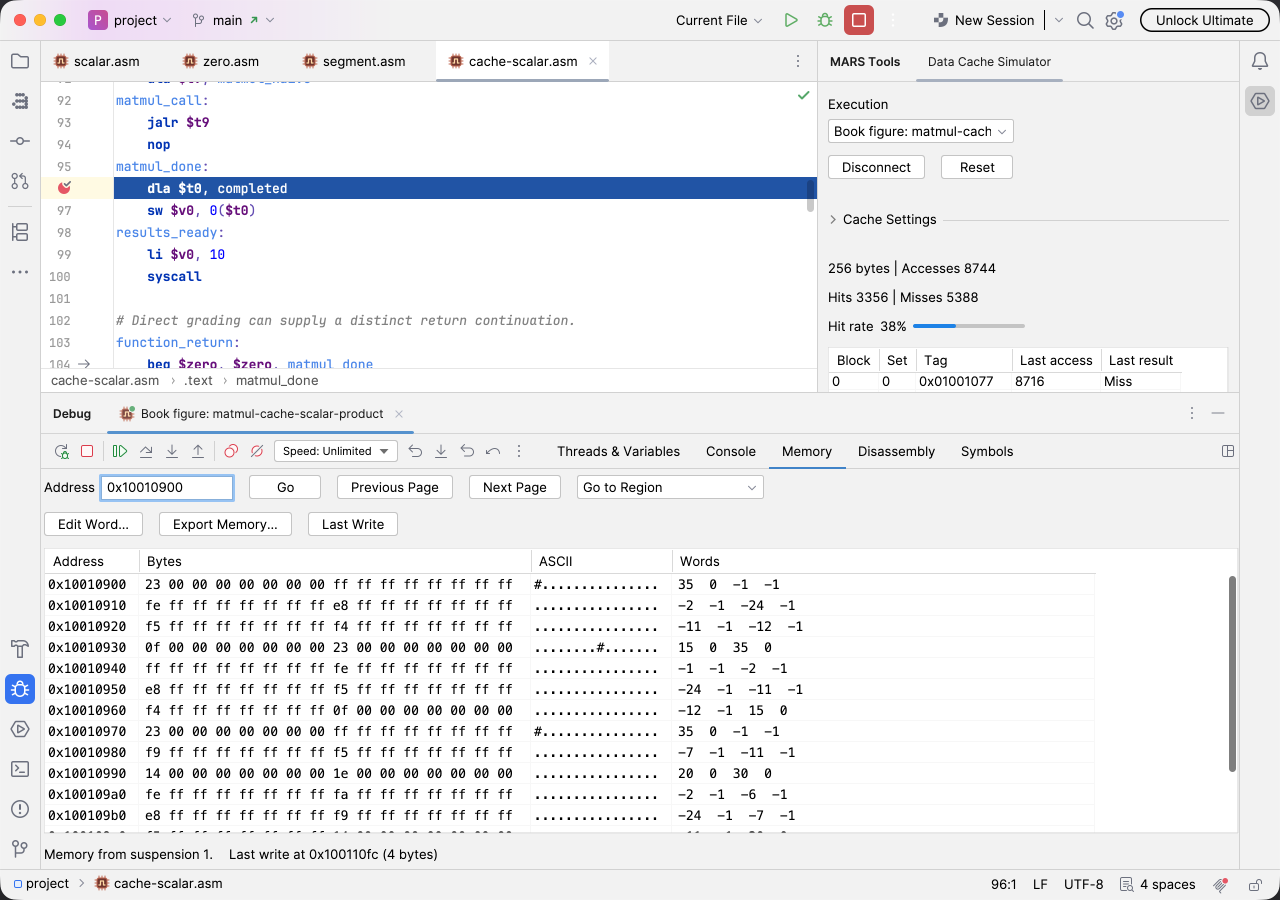
\includegraphics[width=0.84\linewidth,artifact,trim={\MARSmatmulcomparisonscalarproductLeft{} \MARSmatmulcomparisonscalarproductBottom{} \MARSmatmulcomparisonscalarproductRight{} \MARSmatmulcomparisonscalarproductTop{}},clip]{book/captures/022-blocked-matmul/f04/scalar-product.png}};
    \begin{scope}[shift={(scalarproduct.south west)},x={($(scalarproduct.south east)-(scalarproduct.south west)$)},y={($(scalarproduct.north west)-(scalarproduct.south west)$)}]
      \draw[black,line width=0.7pt] (0.194672131,0.055555556) rectangle (0.997950820,0.638888889);
      \node[draw=black,fill=white,circle,inner sep=1.5pt,font=\footnotesize] at ($(0,0.638888889)+(-3mm,0)$) {3};
    \end{scope}
    \node[anchor=north west,inner sep=0,font=\small\bfseries] (tiledproduct-title) at ([yshift=-1mm]scalarproduct.south west) {Tile-four output detail};
    \node[anchor=north west,inner sep=0] (tiledproduct) at ([yshift=-1mm]tiledproduct-title.south west) {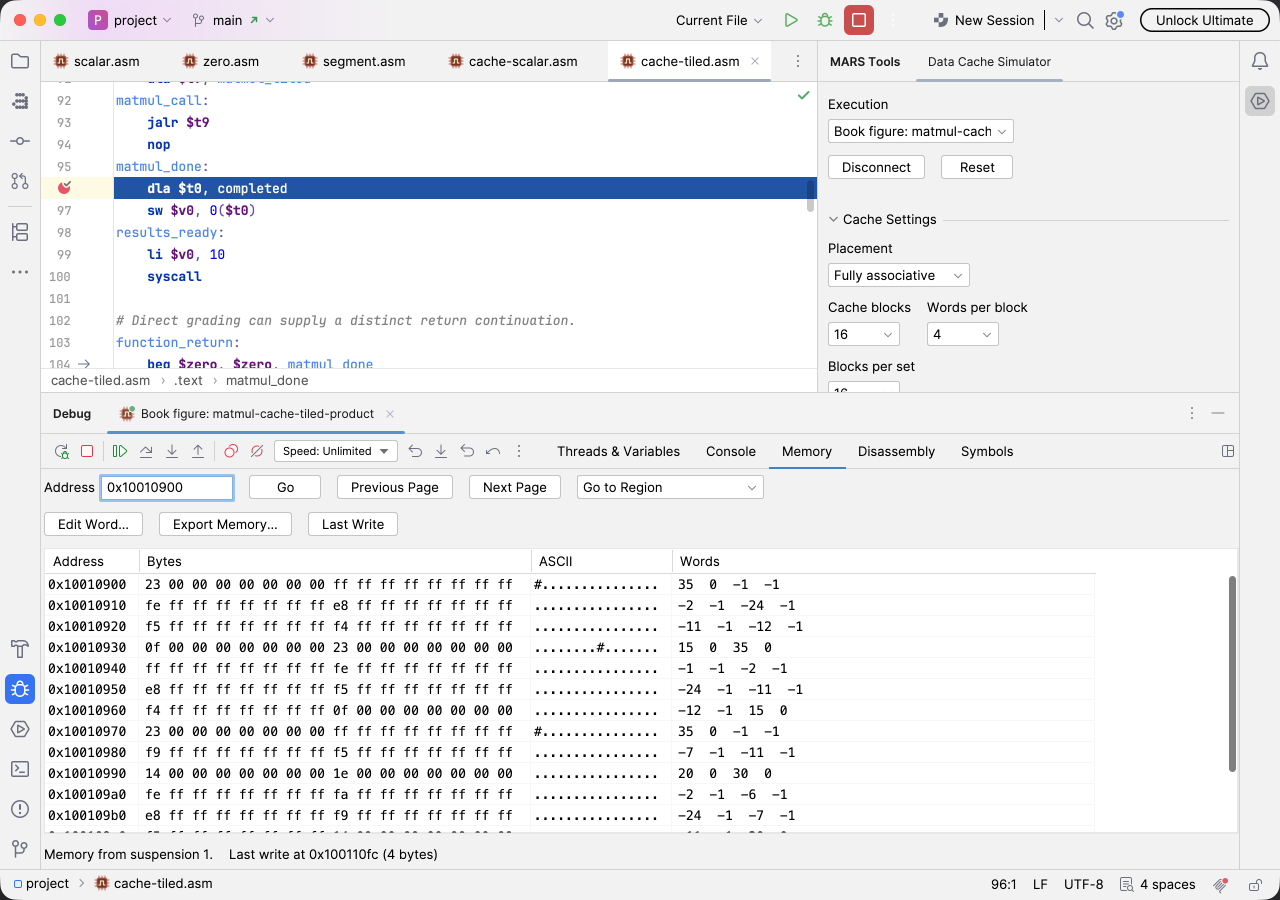
\includegraphics[width=0.84\linewidth,artifact,trim={\MARSmatmulcomparisontiledproductLeft{} \MARSmatmulcomparisontiledproductBottom{} \MARSmatmulcomparisontiledproductRight{} \MARSmatmulcomparisontiledproductTop{}},clip]{book/captures/022-blocked-matmul/f04/tiled-product.png}};
    \begin{scope}[shift={(tiledproduct.south west)},x={($(tiledproduct.south east)-(tiledproduct.south west)$)},y={($(tiledproduct.north west)-(tiledproduct.south west)$)}]
      \draw[black,line width=0.7pt] (0.194672131,0.055555556) rectangle (0.997950820,0.638888889);
      \node[draw=black,fill=white,circle,inner sep=1.5pt,font=\footnotesize] at ($(0,0.638888889)+(-3mm,0)$) {4};
    \end{scope}
  \end{tikzpicture}
  \par\smallskip
  \begin{minipage}{\linewidth}
    \small
    \begin{enumerate}
      \setlength{\itemsep}{2pt}
            \setlength{\parsep}{0pt}
      \item The scalar cache reports 8744 notices, 3356 hits and 5388 misses. Both runs use full associativity, sixteen blocks, four words per block and LRU: 256 bytes, initially cold. The complete capture receipts verify the settings.
      \item Tile four reports 12840 notices, 11772 hits and 1068 misses. The displayed 38 and 92 percent hit rates are rounded. Frame, descriptor and matrix traffic are included; more notices accompany fewer misses.
      \item The scalar output detail shows its first four signed doublewords: $35,-1,-2,-24$. Negative values have all-one high words. Every one of the 256 cells is checked, including cells outside this detail.
      \item The tiled output agrees cell for cell. Whole-call counts are 41571 scalar instructions and 59419 tiled instructions, verified separately. Doubleword operations contribute two word notices each. These counters establish neither elapsed time nor processor cycles.
    \end{enumerate}
  \end{minipage}
  \caption{Tile four reduces fully associative misses while increasing notices and instruction work.}
  \label{capture:022-blocked-matmul-f04}
  \label{matmul-f04}
\end{figure}
\par
